\documentclass{article}
\usepackage[utf8]{inputenc}
\usepackage{amsmath}
\usepackage{amsthm}
\usepackage[margin=20px]{geometry}
\usepackage{graphicx}
\usepackage{enumitem}
\usepackage{xcolor}
\setlength{\parindent}{0pt}
\setlist{itemsep=0.02em, topsep=0.3em}

\title{Data Fundamentals}
\author{}
\date{}

\begin{document}

\subsection*{Arrays \small\textcolor{gray}{Week 1}}

\textbf{Basic Concepts}
2 $\times$ 3 means 2 rows, 3 columns.
Rank 1 tensor is 1D array.

\textbf{Concatenate} to join along existing dimension.

\textbf{Stack} to stack up arrays along new dimension.

\textbf{Tiling} to repeat an array.

\begin{itemize}
    \item Starting with two 1D arrays of shape (3,)
    \item Concatenating them creates a single 1D array of shape (6,)
    \item Stacking them creates a 2D array of shape (2, 3)
    \item Stacking with axis = 1 creates a 2D array of shape (3, 2)
\end{itemize}

\textbf{Broadcasting}: You can broadcast an array of shape (x, y) with (x, y), (1, y), (x, 1), (y,).

\textbf{Reduction}: apply a function to reduce the array to a single value or with axis to reduce along a specific axis.

\textbf{Accumulate}: apply a function to reduce the array to a single value.

\textbf{NumPy Functions}
\begin{itemize}
    \item \texttt{np.random.uniform}, \texttt{np.random.normal}, \texttt{np.random.randint}, \texttt{np.random.choice}, \texttt{np.random.permutation}
    \item \texttt{np.tile}, \texttt{np.stack}, \texttt{np.concatenate}, \texttt{np.squeeze}, \texttt{np.reshape}, \texttt{np.einsum}, \texttt{np.ravel}, \texttt{np.swapaxes}, \texttt{np.rollaxes}
\end{itemize}

\subsection*{Floats \small\textcolor{gray}{Week 2}}

\textbf{Float Exceptions}

Invalid operation, divide by zero, overflow, underflow, inexact.

Use \texttt{np.allclose} to check if two floats are close.

\textbf{Representation}

$float = sign * 2^{exponent} * mantissa$.

\texttt{float64}: 1 bit for sign, 11 bits for exponent, 52 bits for mantissa.

\texttt{float32}: 1 bit for sign, 8 bits for exponent, 23 bits for mantissa.

\texttt{inf} is represented with all 1s in the exponent and 0s in the mantissa.

\texttt{nan} is represented with all 1s in the exponent and non-zero in the mantissa.

\textbf{Strides}

Stride: number of bytes between each element in an axis.

To find the element at index [i, j, k] in a numpy array, we need to know the shape of the array and the strides.

\texttt{strides = (shape[0] * itemsize, shape[1] * itemsize, shape[2] * itemsize)}

\texttt{element = base + i * strides[0] + j * strides[1] + k * strides[2]}

\textbf{Dope vectors}: Hold striding information.

\textbf{Illife vectors}: Holds nested pointers to other arrays / values.

To transpose a 2D array, we need to reverse the swap then dimensions and swap the strides.

\textbf{Rank and Dimensions}

\textbf{Add singleton dimensions}: \texttt{x[:, np.newaxis]} or \texttt{x[:, None]}

\textbf{Remove singleton dimensions}: \texttt{np.squeeze}

\textbf{Elided axes}: \texttt{[0, \ldots, 4]}

\textbf{Swapping and rearranging}: \texttt{np.swapaxes, np.rollaxis, np.moveaxis, np.transpose}

\textbf{Einsum}: Einstein summation convention. Used to reorder high-dimensional arrays.

\clearpage

\subsection*{Scientific Visualisation \small\textcolor{gray}{Week 3}}

\textbf{Basic Terminology}

A \textbf{stat} is a statistic computed from data, such as means (mean, median, max, min,  etc.)

A \textbf{mapping} represents a transformation of data attributes to visual values. It maps stats using a scale to give units.

A \textbf{guide} is a visual reference which indicates the meaning of a mapping. Axes which are labeled are guides for the coordinate system.
Legend is a guide for the mapping. A grid is a guide for the coordinate system.

A \textbf{geom} is the geometric representation of data after it has been mapped. Lines, markers, patches, bars.

A \textbf{coord} is a coordinate system, which connects mapped data onto points on a plane.

A \textbf{layer} of a plot is one set of geoms, with one mapping on one coordinate system.

A \textbf{facet} is a different view on the same dataset, on a separate coordinate system.

A \textbf{figure} comprises a set of one or more facets

A \textbf{caption} explains the visualization to the reader.

A \textbf{scale} specifies how units are transformed.

\vspace{\baselineskip}

\textbf{Stats}

Avoid rescaled units. This can be misleading.

\textbf{Regression}: fit a line to the data.

\textbf{Smoothing}: fit a curve to the data.

\textbf{Aggregate summary statistics}: statistics which summarise some larger dataset compactly, like the mean.

\textbf{Smoothing and regression} finding simple, smooth functions which approximate observed data.

\textbf{Rank plot}: a plot of values arranged in rank order.

\vspace{\baselineskip}

\textbf{Geoms}

\textbf{Markers}: geoms that represent bare points, typically use as a visual record of a discrete. Can also be used to represent another variable, you
could modify the colour or scaling

\textbf{Colour changes}: percaptually uniform, monotonic brightness, consider if it will be seen in black and white.

Geometric representations, or \textbf{geoms}, that connect points together should be used if it makes sense to ask what is between two data points.
\textbf{Line styles} can have variable thickness, variable color, and dash patterns to enhance the visual representation of the data.

\textbf{Colour maps} should be perceptually linear, monotonic, and continuous.
If your data is signed, use a coloujr map which diverges around 0, and is monotonic in brightness in each side of 0.

For example, the staircase plot is useful when we know that the value cannot have changed between measurements (e.g., in a coin toss scenario).
This type of plot connects points but keeps the value fixed until a new data point is observed.
Conversely, if measurements are naturally discrete, a bar chart may be more suitable to represent the data effectively.

\textbf{Alpha and transparency}

A \textbf{geom} can be rendered with different levels of transparency, referred to as \textbf{alpha} (equivalent to opacity) or
\textbf{transparency} (the inverse of opacity). This feature is particularly useful when dealing with a large number
of overlapping geoms, as it allows for the emphasis of certain geoms while maintaining visibility of others.
However, it is important to use transparency judiciously, as excessive transparency can make graphs difficult to read.

\vspace{\baselineskip}

\textbf{Coords}

\textbf{Aspect Ratio} can be very important, images should never be stretched or squashed.

\textbf{Log scales} can be useful when datasets span orders of magnitude.

\textbf{Symlog} modified logarithmic scale to allow for negative values.

\textbf{Polar coordinates} visual coordinates in terms of angle and distance.

\textbf{Double axes} two different y units overlaid on the same facet.

\textbf{Standard deviation} the average deviation from the average.

\textbf{Nonparametric intervals} intervals based on summary statistics of data, like the interquartile range.


\vspace{\baselineskip}

\textbf{Facets and Layers}

\textbf{Distinct layers} superimposed on the same set of coords.
\textbf{Distinct facets} on separate sets of coords.


\begin{figure}[h]
    \centering
    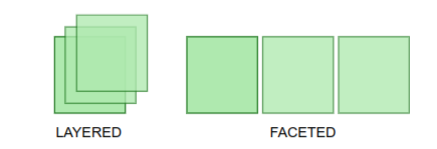
\includegraphics[width=0.2\textwidth]{assets/layered-faceted.png}
    \caption{Layered and Faceted}\label{fig:layered-faceted}
\end{figure}

\vspace{\baselineskip}

\textbf{Communicating Uncertainty}

\textbf{Error Bars} can be shown as the \textbf{standard deviation}, \textbf{standard error}, \textbf{confidence interval}, or \textbf{nonparametric interval}.


\clearpage

\subsection*{Linear Algebra \small\textcolor{gray}{Week 4}}


\textbf{Weighted Sums of Vectors}
$\lambda_1 \mathbf{x}_1 + \lambda_2 \mathbf{x}_2 + \cdots + \lambda_n \mathbf{x}_n$
\textbf{Linear interpolation}
$lerp(x_1, x_2, \alpha) = (1 - \alpha)x_1 + (\alpha)x_2$

\textbf{Norms}
$\|x\|_p = {(\sum_{i=1}^{n} |x_i|^p)}^{\frac{1}{p}}$
$\|x\|_\infty = \max_{i=1}^{n} |x_i|$
$\|x\|_{-\infty} = \min_{i=1}^{n} |x_i|$
\textbf{Normalisation} $x' = \frac{x}{\|x\|_p}$

\textbf{Cosine Distance}
$\cos \theta = \frac{\mathbf{x} \cdot \mathbf{y}}{||\mathbf{x}|| \, ||\mathbf{y}||}$

\textbf{Variance}
$\sigma^2 = \frac{1}{N - 1} \sum_{i=0}^{N-1} {(x_i - \mu)}^2$

\textbf{Covariance Matrices}.
We compute the covariance of every dimension with every other dimension.
$\Sigma_{ij} = \frac{1}{N - 1} \sum_{k=1}^{N} (X_{ki} - \mu_i)(X_{kj} - \mu_j)$.
You can also use $np.cov$.


\subsection*{Linear Algebra 2 \small\textcolor{gray}{Week 5}}

\textbf{Adjacency Matrices} square matrix of $|V| \times |V|$ size (where $|V| =$ vertices) where no edge from $V_i$ to $V_j$ means 0 and existing edges mean 1
\textbf{Out-degree} sum across the rows
\textbf{In-degree} sum across the columns
\textbf{Symmetric matrix} means an undirected graph
directed graph can be turned into an undirected one using: $A` = A + A^T$.
The Laplacian matrix of a graph is $L = D - A$, where $D$ is the degree matrix and $A$ is the adjacency matrix.
$D_{ii} = \sum_{j=1}^{|V|} A_{ij}$
\textbf{A Sparse Matrix} is a matrix with a large number of zero elements, the oppisite is a \textbf{Dense Matrix}.
\textbf{A Stochastic Matrix} is a square matrix of non-negative numbers with each row summing to 1.
\textbf{A Doubly Stochastic Matrix} is a square matrix of non-negative numbers with each row and column summing to 1.
\textbf{Eigenvector} of A is a vector that is only scaled when is applied to it, not rotated.
\textbf{Eigenvalue} of A is how much the eigenvector is scaled by when is applied to it.
$A\vec{x} = \lambda  \vec{x}$.
\textbf{Power Iteration}
$\vec{x_n} = \frac{A \vec{x_{n-1}}}{\|A\vec{x_{n-1}}\|_\infty}$.
$evals, evecs = np.linalg.eigh(A)$.
The \textbf{eigenspectrum} is just the sequence of absolute eigenvalues, ordered by magnitude.

\textbf{Principle Components Analysis}
The eigenvectors of the covariance matrix are called the \textbf{principal components}, and they tell us the
directions in which the data varies most.
The direction of principal component $i$ is given by the eigenvector $\vec{x}_i$, and the length of the
component is given by $\sqrt{\lambda_i}$.

\textbf{The Trace} of a matrix is the sum of its diagonal elements.
\textbf{The Determinant} of a matrix is the product of the eigenvalues: $\text{det}(A) = \prod_{i=1}^n \lambda_i$

\textbf{Positive Definite Matrices}
A matrix is positive definite if all its eigenvalues are greater than zero: $\lambda_i > 0$.

\textbf{Positive Semi-Definite Matrices}
A matrix is positive semi-definite if all its eigenvalues are non-negative: $\lambda_i \geq 0$.

A positive definite mathrix has the property $\vec{x}^T A \vec{x} > 0$ for all nonzero vectors $\vec{x}$.
This tells us that the dot product of $\vec{x}$ with $A \vec{x}$ must be positive
(N.B. $A \vec{x}$ is the vector obtained by transforming $\vec{x}$ with $A$).
This can only happen if the angle $\theta$ between $\vec{x}$ and $A \vec{x}$ is less than $90^\circ$,

Eigenvectors exist only for square matrices.
A matrix $A$ transforms a general vector by rotating and scaling it.
However, the eigenvectors of $A$ are special because they can only be scaled, not rotated by the transform.
The eigenvalues of $A$ are the scaling factors $\lambda_i$ that correspond to each unit eigenvector $\vec{x}_i$.
Eigendecomposition is the process of breaking a matrix down into its constituent eigenvalues
and eigenvectors. These serve as a compact summary of the matrix.
The eigenspectrum is just the list of (absolute) eigenvalues of a matrix, in rank order, largest first.
If we have a complete set of eigenvectors and eigenvalues, we can reconstruct the matrix.
We can approximate a large matrix with a few leading eigenvectors; this is a simplified or
truncated approximation to the original matrix.
If we repeatedly apply a matrix to some vector, the vector will be stretched more and more
along the largest eigenvectors.

\textbf{An orthogonal matrix} is a square matrix with orthonormal columns, $A^T = A^{-1}$.

\textbf{Key Algorithm I\@: Singular Value Decomposition}
A general approach to decomposing any matrix A.
$A = U \Sigma V^T$

$U$ is a \textbf{square unitary mxn matrix}, whose columns contain the left singular vectors,
$V$ is an \textbf{square unitary nxn matrix}, whose columns contain the right singular vectors,
$\Sigma$ is a \textbf{diagonal mxn matrix}, whose diagonal contains the singular values

A \textbf{unitary matrix} is one whose conjugate transpose is equal to its inverse.
The SVD is the same as:
Taking the eigenvectors of $A^T A$ to get $U$
Taking the square root of the absolute value of the eigenvalues $\lambda_i$ of $A^T A$ to get $\Sigma_i = \sqrt{\lambda_i}$
Taking the eigenvectors of $A A^T$ to get $V^T$
$A^n = V \Sigma^n U^T$

\textbf{Pseudo-inverse}
We can also pseudo-inverse a matrix A+ even if A is not square.
$A^+ = V \Sigma^{-1} U^T$

the \textbf{Rank} of a matrix is the number of non-zero singular values,
or the number of linearly independent rows or columns.

The \textbf{condition number} of a matrix is the ratio of the largest singular value to the smallest.

\textbf{Whitening} removes all linear correlations within a dataset.
$X^{\text w} = (X - \vec{\mu}) \Sigma^{-1/2}$ where $\vec{\mu}$ is the mean vector, i.e.
A row vector containing the mean of each column in $X$, and $\Sigma$ is the covariance matrix.

\clearpage

\subsection*{Optimisation \small\textcolor{gray}{Week 6}}

\textbf{Paremeters} are things we can adjust (inputs), they exist in a parameter space: the set of all possible values.

\textbf{Objective Function} (loss function) maps the parameters onto a single numerical measure of how good the configuration is.
The desired output of the optimisation algorithm is the parameter configuration that minimises the objective function.
$\theta^* = \arg \min_{\theta \in \Theta} \text{L}(\theta)$

\textbf{Constraints} are limitations on the parameters. This defines a region of the parameter space that is feasible,
the feasible set or region.

It is common to have express problems in a form where the objective function is a distance between an output
and a reference is measured.

\textbf{Evaluating the objective function} may be expensive, so a good optimisation algorithm will find the optimal
configuration with few queries.

\textbf{Discrete and continuous} optimisation are inferred based on the parameter space.

\textbf{Constraint types}: box constraint, convex constraint (collection of inequalities).
equiality and inequality constraint.

\textbf{Constrained optimisation} could speed it up, though fewer algorithms are available for optimisation.
May be hard to specify feasible region.

\textbf{Soft constraints} work by applying penalties to the objecive function to `discourage' solutions that violate the constraints.

$ L(\theta) = L(\theta) + \lambda C(\theta) $ where $C(\theta)$ is a penalty function with an increasing value as the
constraints are more egregiously violated. $\lambda$ is a penalty coecient that controls how much the constraints are penalised.
This may not respect important constraints.

\textbf{Relaxation} is a technique where an algorithm tries to find a continuous or unconstrained
optimisation problem to solve instead of a discrete optimisation.

\textbf{Penalisation} refers to terms which augment an objective function to minimise some other property of
the solution, typically to approximate constrained optimisation.

\textbf{Properties of the objective function}. A local minimum is any point where the objective function
increases in every direction around that point. An objective function is \textbf{convex} if it has a single, global minimum.

\textbf{Convex optimisation}

\textbf{Algorithms}:
\textbf{Direct convex optimisation} techniques, such as least squares,
are used to find the best-fitting solution by minimizing the sum of the squares of the differences
between observed and predicted values. This method is particularly effective for linear regression
problems, where the goal is to determine the linear relationship between variables.

\textbf{Iterative optimisation}
Make a guess, if the guess is better than the previous guess, keep it, continue until you have reached a good enough solution.
\begin{enumerate}
    \item choose a starting point $x_0$
    \item while objective function changing
    \begin{enumerate}
        \item adjust parameters
        \item evaluate objective function
        \item if better solution found than any so far, record it
    \end{enumerate}
    \item return best parameter set found
\end{enumerate}

\textbf{Grid search}: The parameter space is split equally in each dimension.
This is very slow as it scales with more dimensions.
If the grid is not fine enough, minima can be missed.

\textbf{Hyperparameters} are properties which affect the way in which the optimiser finds a solution.

\textbf{Simple stochastic: random search}: Guess a number $\theta$, check the objective function,
if $L(\theta) \le L(\theta^*)$, then $\theta^* = \theta$.

\textbf{Metaheuristics}:
There are a number of meta-heuristisc that can be used to improve random search.
\textbf{Locality} which takes advantage of the fact the objective function is likely to have similar values for similar parameter configurations.
\textbf{Temperature} which can change the rate of movement in the parameter space over the course of an optimisation.
\textbf{Population} which can track multiple simultaneous parameter configurations and select among them
\textbf{Memory} which can record good or bad steps in the last and avoid them.

\textbf{Hill climbing} is a modication of random search, taking steps up hill to get out of local minimum

\textbf{Simulated annealing} extends hill-climbing with the ability to sometimes randomly go
uphill, instead of always going downhill. It uses a \textbf{temperature schedule} that allows more
uphill steps at the start of the optimisation and fewer ones later in the process. This is used
to overcome ridges and avoid getting stuck in local minima.

\textbf{Population}: track multiple simultaneous parameters configurations and select/mix among them.
Involves mutation (random variables), natural selection (solution selection) and breeding (interchange between solutions).
each iteration will move solutions slightly by random mutation, cull the weakest solutions and copy the remaining “fittest” solutions to keep the population size constant

\textbf{Memory} This ineciency can be mitigated
using some form of memory, where the optimiser remembers where “good” and “bad” bits
of the parameters space are, and makes decisions using this memory. In particular, we want
to remember good paths in solution space.

\textbf{Convergence}
An optimisation algorithm is said to converge to a solution
What can go wrong? Slow progress. Noisy and diverging performance. Getting stuck


% Week 7

\subsection*{Optimisation 2}

\textbf{Gradients of Vector-Valued Functions}.
\textbf{Jacobian}: matrix of partial derivatives.
\textbf{Gradient Vector}: gradient of a scalar-valued function of a vector variable.
\textbf{Hessian}: matrix of second partial derivatives.
\textbf{Lipschitz continuous}: a function $f$ is Lipschitz continuous if there exists a constant $L$ such that for all $x$ and $y$, $|f(x) - f(y)| \leq L |x - y|$.

\textbf{Gradient Descent}: An iterative optimisation algorithm that uses the gradient of the objective function to find a local minimum. The update rule is:
$\theta_{t+1} = \theta_t - \alpha \nabla L(\theta_t)$. While gradient descent can be very fast, following the gradient is not necessarily the fastest route to a minimum.

\textbf{Adaptive Step Sizes}:
\textbf{Line search}: Start with a big step, then reduce it if the gradient is not decreasing.
\textbf{Adagrad}: adapt the step size for each dimension based on the history of the gradient in that dimension.

\textbf{Stochastic Gradient Descent}: If the objective function can be broken down into
small parts, then the gradient can be approximated by sampling the gradient at random points.

\textbf{Eigenvalues of the Hessian}: The Hessian matrix captures important properties about the type of critical
point that we saw in the previous lecture. In particular, the eigenvalues of the Hessian tell us what kind of point we have.
If all eigenvalues are strictly positive, the matrix is called positive definite and the point is a minimum. If all eigenvalues
are strictly negative, the matrix is called negative definite and the point is a maximum. If eigenvalues have mixed signs,
the point is a saddle point. If the eigenvalues are all positive or negative, but with some zeros, the matrix is semidefinite
and the point is a plateau or ridge.


% Week 8

\subsection*{Probability}
\textbf{Experiment/Trial}: An occurrence with an uncertain outcome (e.g., submarine location)
\textbf{Outcome}: Result of an experiment (e.g., submarine in grid [2,3])
\textbf{Sample Space}: Set of all possible outcomes
\textbf{Event}: Subset of possible outcomes with common property
\textbf{Probability}: Ratio of event outcomes to total outcomes (0 to 1)
\textbf{Probability Distribution}: Mapping of outcomes to probabilities that sum to 1
\textbf{Random Variable}: Variable representing unknown value with known probability distribution
\textbf{Probability Density/Mass Function}: Function defining probability distribution
\textbf{Observation}: Directly observed outcome (data)
\textbf{Likelihood}: How likely an observation is given a probability distribution
\textbf{Sample}: Simulated outcome from a probability distribution
\textbf{Expectation}: Average value of a random variable


\textbf{Probability Mass Function}: A function that maps each possible outcome of a discrete random variable to its probability.
\textbf{Probability Density Function}: A function that maps each possible outcome of a continuous random variable to its probability.


\textbf{Expected Value}: The average value of a random variable. For discrete $X$:
$ E[X] = \sum_{x} x \cdot P(x) $
For continuous $X$:
$ E[X] = \int_{-\infty}^{\infty} x \cdot f(x) \, dx $

\textbf{Variance}: A measure of the spread of a random variable's values. For a random variable $X$ with expected value $E[X]$, the variance is defined as:
$ \text{Var}(X) = E[(X - E[X])^2] $


\textbf{Joint Probability}: The probability of two events occurring together. For events $A$ and $B$, the joint probability is:
$ P(A \cap B) = P(A) \cdot P(B|A) $

\textbf{Conditional Probability}: The probability of an event given that another event has occurred. For events $A$ and $B$, the conditional probability of $A$ given $B$ is:
$ P(A|B) = \frac{P(A \cap B)}{P(B)} $

\textbf{Odds}: The ratio of the probability of an event occurring to the probability of it not occurring. For event $A$, the odds are:
$ \text{odds}(A) = \frac{P(A)}{1 - P(A)} $

\textbf{Log-odds} are particularly useful for very unlikely scenarios.

\textbf{Bayes' Theorem}: A fundamental theorem in probability that describes how to update the probabilities of hypotheses when given evidence. The theorem is stated as:
$ P(A|B) = \frac{P(B|A) \cdot P(A)}{P(B)} $.
\textbf{Posterior}: What we want to know after computation
\textbf{Likelihood}: Probability of evidence given the event
\textbf{Prior}: Probability of event before evidence
\textbf{Evidence}: Probability of evidence occurring

\textbf{Integration over the evidence}
$ P(A) = \int P(A|B) \cdot P(B) \, dB $

\textbf{Entropy}:
The entropy of a (discrete) distribution of a random variable can be
computed as:
$ H(X) = - \sum_{x} P(x) \log P(x) $
This is just the expected value of the log-probability of a random variable
(the “average” log-probability).

% Week 9

\subsection*{Probability 2}

% What Monte Carlo approaches are, and how expectation can be approximated

\textbf{Monte Carlo Approaches} involve simulating the random variable many times and averaging the results.

% The specific problems of continuous random variables as compared to discrete random variables

\textbf{Problems of Continuous Random Variables}:
Probability of an exact value is 0.
Unlike with discrete variables, you can't estimate the probability density function (PDF) from simple counts,
since each observation has no width and doesn't `fill in' the distribution.
Bayes' Rule is easy to apply to discrete problems but not continuous

% The normal distribution and the central limit theorem

\textbf{Normal Distribution}:
The normal distribution is a continuous probability distribution that is symmetric and bell-shaped.
It is defined by its mean and standard deviation, and is given by the formula:
$ f(x) = \frac{1}{\sigma \sqrt{2\pi}} e^{-\frac{(x-\mu)^2}{2\sigma^2}} $


% What multivariate distributions are

\textbf{Multivariate Distributions} generalise discrete variables to continuous spaces via probability density functions.

% What inference is

\textbf{Inference} is the process of determining parameters of the function generating data by looking at the aftermath.
Different approaches are \textbf{direct estimation}: define functions of observations that will estimate the values of parameters
of distributions directly.
\textbf{Maximum Likelihood Estimation}: use optimisation to find parameter settings that make the observations appear as likely as possible.
\textbf{Bayesian Inference}: use Bayes' Rule to update the probability of a hypothesis as more evidence is gathered.

% What population, parameters, statistics and samples are

\textbf{Population}: The complete set of individuals or items of interest.
\textbf{Parameters}: Numerical characteristics of the population.
\textbf{Statistics}: Functions of the sample data used to estimate parameters.
\textbf{Sample}: A subset of the population used to make inferences.

% How parameters can be estimated from a sample

\textbf{Parameter Estimation}: Using sample data to estimate population parameters.

% How estimators and maximum likelihood estimation work

\textbf{Estimators}: Functions of the sample data used to estimate parameters.
\textbf{Maximum Likelihood Estimation}: use optimisation to find parameter settings that make the observations appear as likely as possible.

% The maximum likelihood algorithm

\textbf{Maximum Likelihood Estimation Algorithm}:
When no closed-form solution exists for parameter estimation, we use optimization to find the parameters that maximize the likelihood of the observed data.
The likelihood function $L(\theta|x)$ depends on the distribution parameters $\theta$.
To perform the optimization, we convert this to a negative log-likelihood function where $\theta^* = \arg \min_\theta L(\theta)$ and $L(\theta) = -\log L(\theta|x_1,...,x_n) = -\sum_i \log f_X(x_i;\theta)$.
For mixture models such as Gaussian mixtures, the probability density function (PDF) is a weighted combination of N normal distributions.
The PDF is given by $f_X(x) = \sum_i \lambda_i n_X(x;\mu_i,\sigma_i)$ where the weights $\lambda_i$ sum to 1.
When fitting these mixtures, we compute the likelihood for each observation by summing the weighted PDFs from each component of the mixture.


% What Bayesian inference involves

\textbf{Bayesian Inference} involves inferring a distribution over possible parameter settings that are compatible with the data, rather than seeking the most likely parameter setting.
It works by inferring a posterior distribution using Bayes' Rule: $P(\theta|D) = \frac{P(D|\theta)P(\theta)}{P(D)}$.
Here, $P(D)$ is the prior belief, $P(\theta)$ is the evidence, and $P(D|\theta)$ is the likelihood function.
The posterior distribution $P(\theta|D)$ needs to be computed for a distribution over $\theta$, not just specific values.
The normalizing constant $P(D) = \int_\theta P(D|\theta)P(\theta)$ is often intractable to compute directly.
To make Bayesian inference tractable, we can use sampling methods or work with relative probabilities only, where $P(\theta|D) \propto P(D|\theta)P(\theta)$.
Bayesian inference can be applied to both continuous and discrete distributions.
However, closed-form computations are typically much more challenging for continuous distributions.

% MCMC approaches to sampling posteriors in Bayesian inference

\textbf{Markov Chain Monte Carlo (MCMC)} samples from difficult probability distributions via random walks in parameter space. It accepts changes that improve likelihood, sometimes accepting worse changes with probability proportional to the likelihood change.
MCMC's key advantage is working with relative probabilities, avoiding normalization constants and complex integrals. It only needs prior and likelihood evaluation for any parameter setting, enabling sampling from any evaluable distribution.
MCMC enables direct model inference without complex approximations or analytical solutions, working purely algorithmically.
However, MCMC has limitations. While asymptotically correct, sampling strategy choice significantly impacts practical performance. Bayesian inference should depend only on priors and evidence, but MCMC results also depend on the sampling strategy.


% The Metropolis-Hastings algorithm

\textbf{Metropolis-Hastings Algorithm}:
The Metropolis-Hastings algorithm is a MCMC method that uses a proposal distribution to generate candidate samples.
It accepts moves that increase the likelihood, and sometimes accepts moves that decrease likelihood with probability
proportional to the likelihood ratio.

% The difference between the posterior and the predictive posterior

\textbf{Posterior Distribution}:
The posterior distribution is the distribution of the parameters given the data.

\textbf{Predictive Distribution}:
The predictive distribution is the distribution of the data given the parameters.


% Week 10

\subsection*{Digital Signals and Time Series}

% what sampling is, for 1D and 2D signals

\textbf{Sampling} is the process of taking measurements of a continuous signal at discrete points in time.
\textbf{Quantisation} means to force something to a discrete set of values.

% how amplitude quantization affects signals

\textbf{Amplitude Quantisation} is the process of converting a continuous amplitude into a discrete set of values.

% what the sampling rate and Nyquist limit are

\textbf{Sampling Rate}: how frequently we have sampled the original data.
\textbf{Nyquist Limit}: the maximum frequency that can be represented in a signal without aliasing.
Usually $f_n = f_s/2$ where $f_s$ is the sampling rate.

% what aliasing is, and how and when it manifests itself

\textbf{Aliasing} is the phenomenon where high frequencies are misinterpreted as lower frequencies.

% the importance of noise and the signal-to-noise ratio

\textbf{Noise} is unwanted information in a signal.
\textbf{Signal-to-Noise Ratio (SNR)} is the ratio of the power of the signal to the power of the noise.

% the purpose of filtering signals

\textbf{Filtering} takes advantage of the fact that we we have temporal structure.
Real signals cannot have arbitrary changes.

% how moving averages work
This idea of a sliding window is critical in digital signal processing. A
sliding window takes a sampled signal of unbounded length, and reduces
it to a collection of fixeded length vectors

% how median filtering works

\textbf{Median Filtering} is a non-linear filtering technique that replaces each pixel with the median value of the pixels in a neighborhood.

\textbf{Linear Filtering} is a filtering technique that uses a linear combination of the pixels in a neighborhood to produce a new pixel.

% how convolution is implemented

\textbf{Convolution} is the process of taking weighted sums of neighbouring values.

% standard types of convolution, including smoothing

\textbf{Smoothing} is a type of convolution that uses a Gaussian kernel to blur the image.

% what the frequency domain and time domain are and what they represent

We can view signals in two ways: as a sequence of amplitude measurements over time: \textbf{the time domain}
,as a sum of oscillations with different frequencies: \textbf{the frequency domain}

% how the Fourier transform relates the time domain to the frequency domain

The Fourier Transform is a mathematical operation that decomposes a signal into its constituent frequencies.

% what convolution is and how the Fourier transform can be used to predict its behaviour

Convolution is the process of taking weighted sums of neighbouring values.
The Fourier Transform can be used to predict the behaviour of convolutions.



\textbf{Frequency Domain Analysis}

Signals can be represented in two ways. In the time domain, we see a sequence of amplitude measurements over time. In the frequency domain, we see a sum of oscillations with different frequencies.

A pure oscillation is represented by a sine wave:
$x(t) = A\sin(2\pi\omega t + \theta)$
where $\omega$ represents the frequency, $\theta$ represents the phase (time offset), and $A$ represents the magnitude.

\textbf{Fourier Transform}

The Fourier Transform decomposes any repeating continuous function into sine waves. It expresses signals as a sum of sinusoidal functions:
$x(t) = \sum_i A_i\sin(\omega_i 2\pi t + \theta_i)$

The correlation between signals is calculated as:
$c = \sum_t a[t]b[t]$
When signals are unrelated, $c$ is approximately 0. For similar signals, $c$ is large and positive, while for inverse signals, $c$ is large and negative.

The phase can be calculated using:
$\theta = \tan^{-1}\left(\frac{c(\omega)}{c'(\omega)}\right)$

The Fourier transform formula is:
$\hat{f}(\omega) = \int_{-\infty}^{\infty} f(x)e^{-2\pi ix\omega}dx$

For real signals, we only need to consider the real part of the complex output.

\textbf{Discrete Fourier Transform (DFT)}

The Discrete Fourier Transform works on discrete measurements. It has complex components representing phase and magnitude. The frequency is calculated as $freq = \frac{f_N k}{N}$. In terms of computational complexity, the DFT requires $O(N^2)$ operations, while the Fast Fourier Transform (FFT) requires only $O(N\log N)$ operations when N is a power of 2.

\textbf{Convolution Theorem}

The Convolution Theorem states:
$FT(f(x) * g(x)) = FT(f(x))FT(g(x))$
where $FT$ represents the Fourier Transform, $*$ represents convolution, and $IFT$ represents the Inverse Fourier Transform.

\textbf{Filter Types}

There are several types of filters. A lowpass filter reduces high frequencies, while a highpass filter reduces low frequencies. A bandpass filter reduces frequencies outside a specific band, and a notch/bandstop filter reduces frequencies inside a band.

Linear filters can only modify existing frequencies, not introduce new ones.




\end{document}